%%%%%%%%%%%%%%%%%%%%%%%%%%%%%%%%%%%%%%%%%%%%%%%%%%%%%%%%%%%%%%%%%%%%%%%%%%%
%
% Plantilla para un artículo en LaTeX en español.
%
%%%%%%%%%%%%%%%%%%%%%%%%%%%%%%%%%%%%%%%%%%%%%%%%%%%%%%%%%%%%%%%%%%%%%%%%%%%



%--------------------------------------------------------------------------
\title{Plantilla para un artículo \LaTeX}
\author{El autor va aquí\\
  \small Dept. Plantillas y Editores\\
  \small E12345\\
  \small España
}

\begin{document}
\section{Resumen}
Los sistemas de recomendaciones son herramientas que generan recomendaciones sobre un determinado objeto de estudio, a partir de las preferencias y opiniones dadas por los usuarios. El uso de estos sistemas se está poniendo cada vez más de moda en Internet debido a que son muy útiles para evaluar y filtrar la gran cantidad de información disponible en la Web con objeto de asistir a los usuarios en sus procesos de búsqueda y recuperación de información. En este trabajo realizaremos una revisión de las características y aspectos fundamentales relacionados con el diseño, implementación y estructura de los sistemas de recomendaciones analizando distintas propuestas que han ido apareciendo en la literatura al respecto.

\section{Abstract}
The recommendation systems are tools that generate recommendations on a specific object of study, based on the preferences and opinions given by the users. The use of these systems is becoming increasingly popular on the Internet because they are very useful for evaluating and filtering the large amount of information available on the Web in order to assist users in their search and information retrieval processes. . In this work we will review the characteristics and fundamental aspects related to the design, implementation and structure of the recommendation systems analyzing different proposals that have appeared in the literature in this regard.

\newpage

\section{Introduccion}
A menudo es necesario seleccionar una entre varias alternativas sin tener un conocimiento exacto de cada una de ellas. En estas situaciones, la decisión final puede depender de las recomendaciones de otras personas [14]. En recuperación de información (RI) los sistemas de recomendaciones (SR) son herramientas cuyo objetivo es asistir a los usuarios en sus procesos de búsqueda de información, ayudando a filtrar los ítems de información recuperados, usando recomendaciones propuestas sobre esos ítems. Dichas recomendaciones se generan a partir de las opiniones proporcionadas por otros usuarios sobre esos ítems en búsquedas previas o bien a partir de las preferencias del usuario objeto de la recomendación (en adelante, usuario activo), dando lugar a los dos grandes grupos de SR [19], los colaborativos y los no colaborativos o basados en contenidos. El uso de estos sistemas se está poniendo cada vez más de moda debido a su utilidad para evaluar y filtrar la gran cantidad de información disponible en la Web para asistir a los usuarios en sus procesos de búsqueda y recuperación de información [9, 11].

Algunos ejemplos reales de SR existentes en Internet son PHOAKS, Referral-Web, Fab, Siteseer, GroupLens, etc., [1, 14]. En todos ellos se manifiesta un claro problema para representar la subjetividad e imprecisión asociadas típicamente a las opiniones o recomendaciones de los usuarios. La Teoría de Conjuntos Difusos constituye un marco de trabajo idóneo para representar la subjetividad e imprecisión a través del modelado lingüístico y los conjuntos difusos [20]. En [10, 19] podemos encontrar algunos SR basados en lógica difusa.

La idea principal de este trabajo es presentar un estudio sobre los SR para la RI en Internet describiendo los aspectos más significativos de su diseño y problemas fundamentales con los que nos encontramos a la hora de diseñar un sistema de este tipo. Analizaremos los elementos que intervienen en el esquema de funcionamiento de un SR y los usaremos como criterios de clasificación.

El trabajo se estructura en cinco secciones. En la Sección 2 presentamos un estudio de los SR en general, presentando distintas taxonomías de SR según los criterios que tengamos en cuenta. En la Sección 3, nos centramos en aspectos de la evaluación de los SR, analizando distintas métricas que se pueden usar. En la Sección 4 proponemos posibles vías de trabajo futuras, para finalizar con nuestras conclusiones en la última sección.


\newpage
\begin{center}
    SISTEMA DE RECOMENDACION DE LIBROS DE BIBLIOTECA
\end{center}
\begin{figure}[htb]
\begin{center}
\includegraphics[width=15cm]{./Imagenes/imagen1}
\end{center}
\end{figure}
\begin{enumerate}
    \item \textbf {Marco Teórico}\\
    Con la finalidad de reflejar los intereses de los usuarios y realizar recomendaciones,los sistemas de recomendación recopilan la información de los usuarios a través delproceso de retroalimentación. Este proceso es la pieza clave para el buen funcionamiento de un sistema de recomendación, porque sin la información recuperada por este, sería imposible conocer el interés de los usuarios y por esto, el sistema tampoco podría recomendarles contenidos interesantes.
    Los sistemas de recomendación también son muy utilizados en el ámbito de las redes sociales. Por ejemplo, YouTube se sirve de un sistema de recomendación para sugerir a los usuarios diferentes vídeos que pueden interesarles según su historial de navegación en el sistema, con lo que se pretende mejorar la experiencia del usuario; Facebook que tiene un sistema de recomendación basado en filtrado colaborativo,que recomienda amigos en base a los amigos que tienen en común los usuarios, estos son algunos ejemplos de redes sociales, pero la gran mayoría de de redes sociales tienen su propio sistema de recomendación integrado.
    Si bien se ha visto que los sistemas de recomendación son ampliamente utilizados en la web, su aplicación en otro tipo de entornos no está tan extendida. Centrándose en el mundo de los libros electrónicos, un sistema que ayude al usuario a seleccionar documentos de su interés de manera automática, sin que tenga que ponerse a buscar entre todo el volumen de libros a los que puede acceder, o que al menos discrimine automáticamente cosas que no le van a interesar, resulta muy atractivo. La tendencia de investigación actual en los sistemas de recomendación es intentar que el sistema llegue a conocer al usuario sin que éste le tenga que dar información explícita sobre sus gustos y preferencias.\\
    
    \textbf{- Definiciones de sistemas de recomendación}\\\\
    A continuación, se presentan diferentes definiciones planteadas por algunos autores sobre sistemas de recomendación. No es el objetivo principal definir este concepto sino mostrar la variedad de definiciones existentes para luego establecer una definición que servirá como marco conceptual para este trabajo:\\
    
    «Un sistema de recomendación es un sistema que tiene como tarea principal,elegir ciertos objetos que cumplen con los requisitos de los usuarios, donde cada unos de estos objetos están almacenado en un sistema informático y caracterizados por un conjunto de atributos.» [Wang, 1998]\\
    «Un sistema recomendador es una tecnología de filtrado de información personalizada, usada para predecir si a un usuario particular le gusta un ítem en particular (problema de predición), o identificar un conjunto de N ítems que pueden interesarles a ciertos usuarios (problema de recomendación top-N.)» [Karypis, 2001]

    
    \textbf{- Sistemas de recomendación basado en contenidos}\\\\
    También se conoce con el nombre de sistema de recomendación no colaborativos y el sistema trata de recomendar productos similares a los que le ha gustado a un usuario determinado en el pasado. Estos productos han sido previamente valorado por el usuario. Para saber que un ítem es parecido a otro se buscan “palabras clave” del ítem que calificó el usuario. Esto puede presentar un problema ya que si siempre se recomiendan ítems similares a los vistos anteriormente se puede llegar a lo que se conoce como sobre-especialización. Un ejemplo de esto, es que si en un sistema de recomendación de películas un usuario solo ha valorado películas de temática o género acción, va a ser difícil que el sistema le recomiende películas de comedia o infantiles. Una de las soluciones posibles es añadiendo algo de aleatoriedad a las recomendaciones del sistema. Los sistemas de recomendación basados en contenidos presentan las siguientes ventajas e inconvenientes [Huecas and Salvachúa, 2010]:\\\\
    \textbf{-Ventajas}\\
    ->Recomendación por contenido y no por opiniones subjetivas de otros usuarios.\\
    -> El sistema puede generar explicaciones sobre la recomendación que hizo en base al historial del usuario

    
    \textbf{- Sistemas de recomendación basados en filtrado colaborativos}\\\\
    También se los conoce con el nombre de sistemas de recomendación colaborativos. Estos tienen como objetivo conocer las preferencias del usuario y hacer recomendaciones sobre la base de datos de los usuarios y la comunidad. El sistema recomienda ítems de otros usuarios con “gustos” similares a los suyos. Por tanto, el sistema de recomendación calcula la similitud entre usuarios y crea lo que llaman “vecinos cercanos” , es decir, usuarios que tienen las mismas valoraciones o calificaciones en los mismos ítems. Por ejemplo, si un usuario calificó 20 ítems y hay otro usuario que coincide en 16 de esas calificaciones, éste sería un “vecino” y es muy probable que los ítems del “vecino” (y que el usuario no valoró) le resulten interesantes. Los sistemas de recomendación basados en filtrado colaborativo presentan las siguientes ventajas e inconvenientes [Huecas and Salvachúa, 2010]:\\
    \textbf{-Ventajas}\\
    - No necesita modelo detallado de preferencias; basta con un vector valoración de objetos\\
    - Permite recomendar contenidos difíciles de analizar.

    
    
    
    \item \textbf {Ejemplos}\\
    En esta sección vamos a analizar algunos ejemplos de SR existentes en Internet [14] que han servido de base para numerosos estudios:\\
    
    \textbf{PHOAKS :} Se trata de un sistema experimental para solucionar el problema de encontrar información relevante y de alta calidad en la Web, usando el enfoque colaborativo en el que los usuarios recomiendan determinados ítems a otros usuarios. PHOAKS trabaja reconociendo, concordando y redistribuyendo automáticamente recomendaciones de recursos Web extraídos de mensajes de noticias.\\
    
    \textbf{Referral Web :} Numerosos estudios muestran que una de las formas más efectivas de divulgar información y conocimientos dentro de una determinada organización es a través de una red informal de colaboradores o amigos. Referral Web se basa en la idea de combinar 'redes sociales' con el filtrado colaborativo, entendiendo por 'redes sociales' grupos de personas vinculadas por determinadas actividades profesionales.\\
    
    \textbf{FAB :} Sistema orientado a la recomendación de URL que combina el uso de información por extensión con el enfoque colaborativo.\\
    
    \textbf{Siteseer :} Recomienda páginas Web relevantes y usa las listas de favoritos y la organización de registros, como una declaración implícita de intereses respecto al contenido subyacente y se va midiendo el grado de solapamiento con las de otros usuarios.\\
    
    \textbf{GroupLens :} El proyecto GroupLens diseña, implementa y evalúa un sistema de filtrado colaborativo para Usenet, un servicio de listas de discusión con un alto volumen de negocio en Internet.\\\\
    definíamos cinco aspectos o dimensiones a considerar a la hora de diseñar un SR. Pues bien, en la tabla 2.2 mostramos cómo se clasifican con respecto a dichos aspectos los sistemas que hemos comentado como ejemplo.\\\\
    Tabla 2.2. Caracterización de algunos SR
    
    \begin{center}
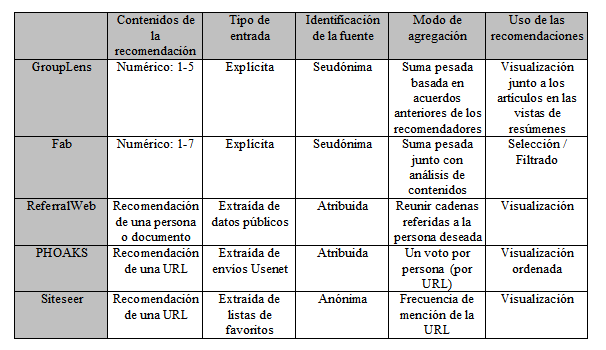
\includegraphics[width=15cm]{./Imagenes/tablas}
\end{center}
    
    \item \textbf {Analisis}\\
    
    
\end{enumerate}


\newpage

\section{Conclusiones}

\begin{itemize}
\item En este trabajo hemos realizado un análisis del paradigma de los SR, como herramientas de gran utilidad de cara a ayudar a los usuarios en sus procesos de búsqueda y recuperación de información. Según el proceso de filtrado en que se basa la generación de recomendaciones, hemos distinguido entre dos grandes grupos de SR, los colaborativos y no colaborativos, llegando a la conclusión de que en muchas ocasiones, la mejor opción es adoptar un enfoque híbrido y así aprovechar las ventajas de ambos. Hemos completado nuestro estudio presentando algunas de nuestras líneas futuras de trabajo para el desarrollo de SR en RI.

\item 


\end{itemize}


\newpage
% Bibliografía.
%-----------------------------------------------------------------
\begin{thebibliography}{99}


\bibitem{Cd94} http://catarina.udlap.mx/u-dl-a/tales/documentos/lis/ramirez-v-m/capitulo2.pdf
\bibitem{Cd94} https://jarroba.com/que-son-los-sistemas-de-recomendacion/ 
\bibitem{Cd94} https://www.upf.edu/hipertextnet/numero-2/recomendacion.html

\end{thebibliography}

\end{document}
